\documentclass[handout, 12pt]{beamer}
\usepackage{pgfpages}
\pgfpagesuselayout{4 on 1}[border shrink=5mm]

\usetheme{Singapore}
%\hypersetup{pdfpagemode=FullScreen}

\title{Introduction to Philosophy}
\subtitle{Lecture 4}

\date{January 30, 2014}
\author{Dr. Scott O'Connor}

\institute{University of Maryland, Baltimore County}





\AtBeginSection{\frame{\sectionpage}}
\AtBeginSubsection{\frame{\subsectionpage}}
\AtBeginSubsubsection{\frame{\subsubsectionpage}}


\begin{document}





\section{Recap}

\frame{
 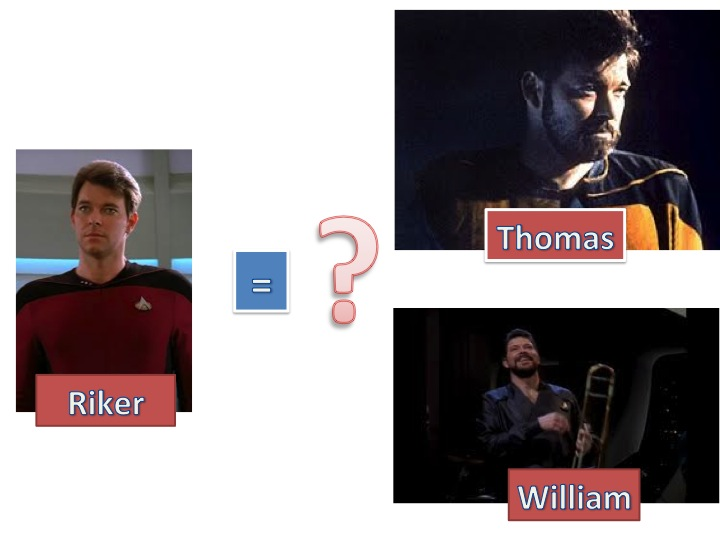
\includegraphics[width=\textwidth]{Slide1.jpg}
}


\frame{\frametitle{What does personal identity consist in?\\Three Options}


 \begin{block}{Same Body Theory}
A person A at one time is identical to  a person B at a later time iff the body of A is identical to the body of B. \pause   
\end{block}
\begin{block}{Same Soul Theory}
A person A at one time is identical to  a person B at a later time iff the soul of A is identical to the soul of B. \pause
\end{block}
\begin{block}{Psychological Continuity Theory}
A person A at one time is identical to a person B
at a later time iff B is psychologically continuous with A.
 \end{block}
 }

\frame{\frametitle{Further Clarification of our Question}
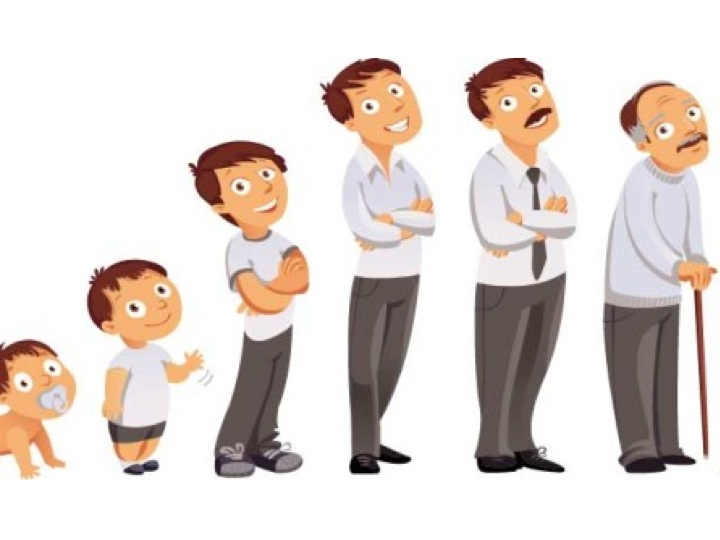
\includegraphics[width=\textwidth]{stages.jpg}
}

\frame{\frametitle{Appropriate Connection: Example}
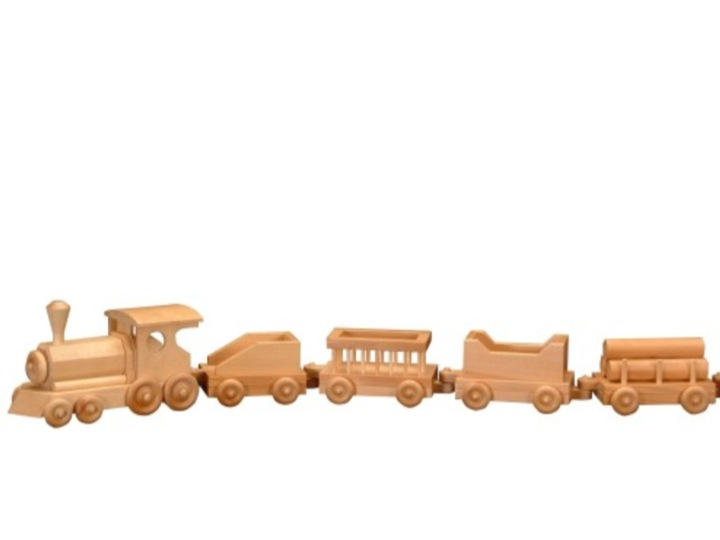
\includegraphics[width=\textwidth]{train.jpg}
}

\section{Version 1}

\frame{\frametitle{Memory Continuity}

A person A at one time is identical to a person B
at a later time iff B \emph{remembers} the \emph{experiences} that A has. 

}



\frame{\frametitle{Memory}


\begin{block}{Factual Memories} Memories that a particular event occurred. They can be shared by several people, e.g., many of us remember President Obama's inauguration.
\end{block}
\begin{block}{Personal Memories} Memories of having the experience of an event. They cannot be shared, e.g., only President Obama has the memory of \emph{being inaugurated} at his inauguration. 
\end{block}

}

\frame{
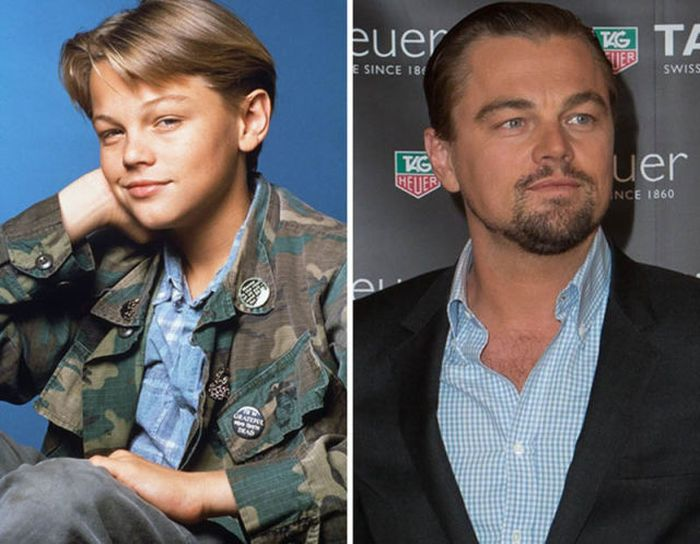
\includegraphics[width=\textwidth]{leo.jpg}
}
\frame{\frametitle{Objection}

\begin{itemize}
\item Allow `Rike' to be the 7 year old who will grow up to be Riker.
\begin{itemize}
\item[P1] Riker = Rike only if Riker remembers everything that Rike experenced. 
\item[P2] Riker does not remember what Rike ate for breakfast on the second day after his 7th birthday, though Rike certainly had the experience of eating something
\item[C] Riker $\neq$ Rike
\end{itemize}
\end{itemize}
}

\section{Version 2}

\frame{\frametitle{Psychological Continuity-Version 2}

A person A at one time is identical to a person B
at a later time iff B is psychologically continuous with A.

\begin{block}{Psychological Continuity}
There is a chain of person-stages connected by
episodic memory.
\end{block}
}

\frame{\frametitle{Psychological Continuity}

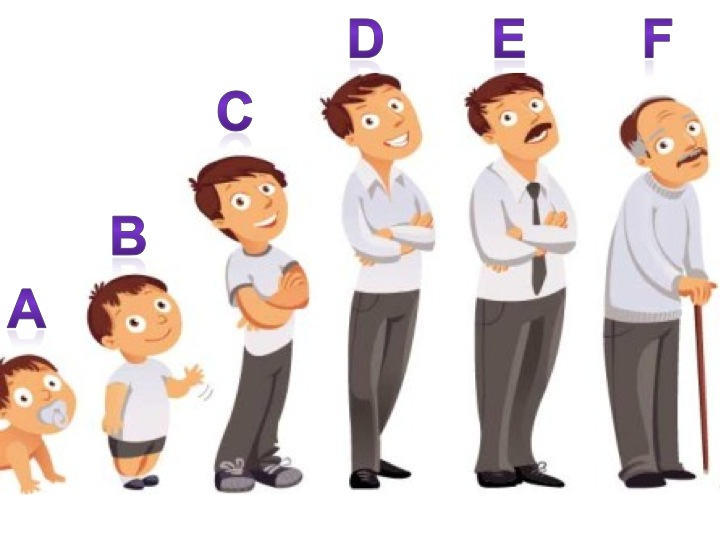
\includegraphics[width=\textwidth]{letters.jpg}

}
\frame{
\begin{itemize}
\item F remembers what E experienced.
\item E remembers what D experienced.
\item D remembers what C experienced.
\item C remembers what B experienced.
\item B remembers what A experienced.
\item Thus, A, B, C, D, E, and F are psychologically continuous with each other. 
\item Hence, they are all stages of the one very same person.
\end{itemize}
}

\frame{\frametitle{River Objection}
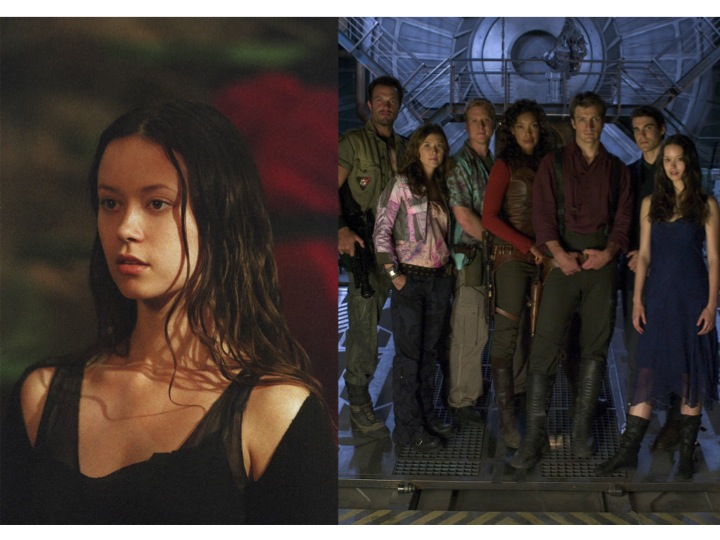
\includegraphics[width=\textwidth]{river.jpg}
}
\frame{\frametitle{Problem: Apparent vs Real Memory}
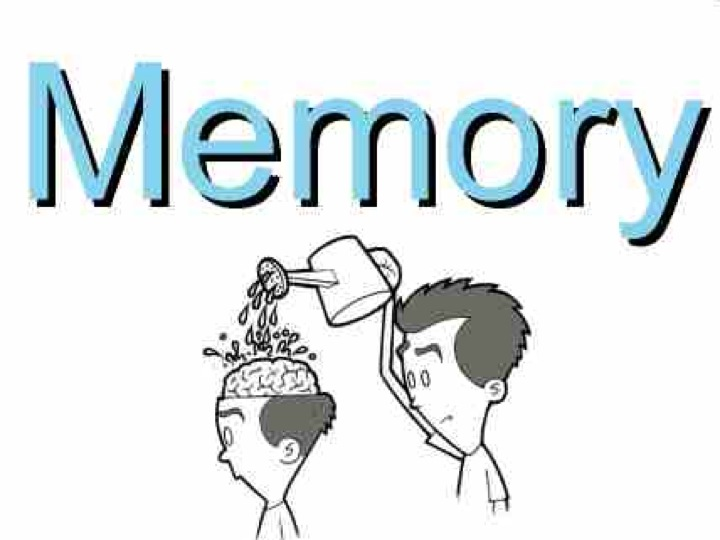
\includegraphics[width=\textwidth]{fake.jpg}
}

% false memory syndrome-false memories of traumatic experiences.
%Misinformation effect - experience that x is P. Someone tells you things about P and it changes your memory of x. 
% Rich false memories - not just distorted memories of what happened, memories of things which never happened. 
% 




\frame{

\begin{block}{I really remember X iff}
\begin{itemize}
\item I have an experience as though I
remember experiencing X.
\item I did experience X.
\end{itemize}
\end{block}

\begin{block}{I apparently remember X iff}
\begin{itemize}
\item I have an experience as though I remember experiencing X.
\item I did not experience X.
\end{itemize}
\end{block}
}


\frame{\frametitle{Distinguishing Real vs. Apparent Memories: Attempt 1}

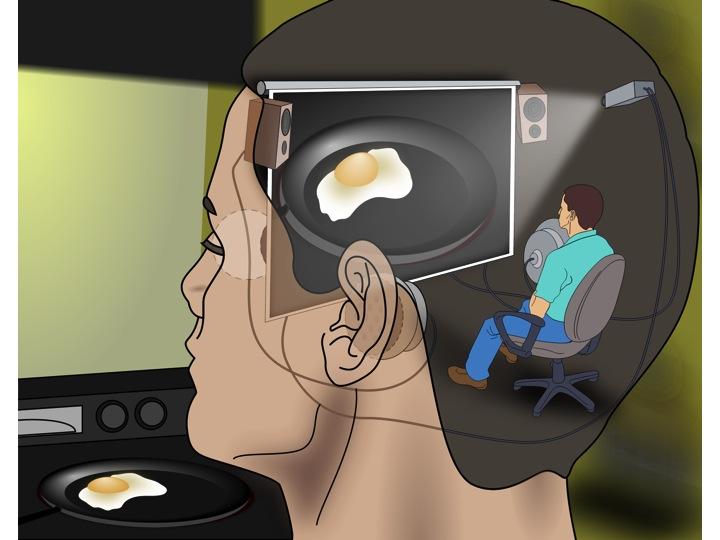
\includegraphics[width=\textwidth]{seat.jpg}

}

\frame{\frametitle{Internal Differences}

\begin{itemize}
\item[P1] If I could perceive a qualitative difference between a real and an apparent memory of X, then this qualitative difference would distinguish the real and apparent memory of X.
\item[P2] I can perceive no qualitative difference between a real and an apparent memory of X.
\item[C] No qualitative difference distinguishes real and apparent memories of X. 
\end{itemize}

}

\frame{\frametitle{Distinguishing Real vs. Apparent Memories: Attempt 2}

\begin{block}{Suggestion:}
If two persons A and B both have an experience as though they remember the experiences of some person P, then the memory of A (or B) is real and not apparent only if A (or B) is identical to P. 
\end{block}
\begin{block}{The problems is that it is circular to make both claims:}
\begin{enumerate}
\item A = P only if A really remembers what P experiences. 
\item A really remembers what P experiences only if A = P. 
\end{enumerate}
\end{block}
}

\frame{\frametitle{Circular Reasoning}

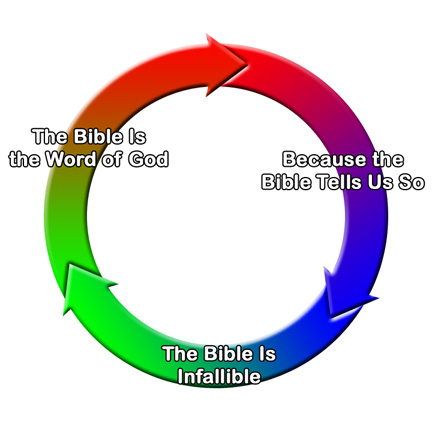
\includegraphics[width=\textwidth, height=\textheight]{circularity.jpg}

}

\frame{\frametitle{Distinguishing Real vs. Apparent Memories: Attempt 3}

\begin{block}{Suggestion}
\begin{itemize}
\item A real memory is one that was caused in the right way.
\item An apparent memory is one that was not caused in the right way, e.g. hypnosis, implantation, etc.\pause
\end{itemize}
\end{block}
\begin{block}{Problem-Duplicates!}
\begin{itemize}
\item[P1] Two persons A and B both have memories of what P experienced that were caused in the right way.
\item[P2] A $\neq$ B.
\item[C] Having memories caused in the right way is not sufficient for personal identity.
\end{itemize}
\end{block}
}
\frame{\frametitle{Riker Objection}
 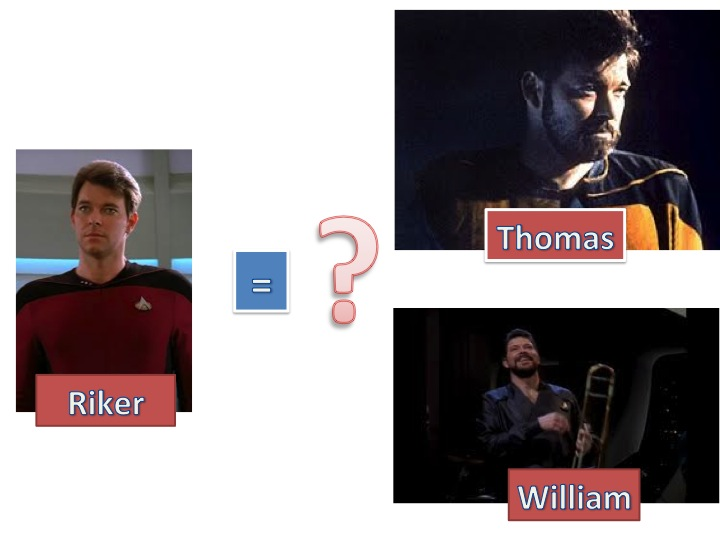
\includegraphics[width=\textwidth]{Slide1.jpg}
}

\end{document}









 

